% EPL master thesis covers template
\documentclass{EPL-master-thesis-covers-EN}

% \documentclass{article}
% \usepackage[utf8]{inputenc}
% \usepackage{float}
% \usepackage{graphicx}
\usepackage{tikz}
\usepackage[demo]{graphicx}
% \usepackage{subcaption}
\usepackage{pgfplots}
\usepackage{enumitem}
\usepackage{amsmath}

\usepackage{graphicx}
\usepackage{float} 
\usepackage{subfigure}
\usepackage[justification=centering]{caption}
% \usepackage{lineno}
% \linenumbers



% Please fill in the following boxes
% Title of the thesis
\title{Large-scale data visualization with BH t-SNE, LargeViz, and Umap}

% Subtitle - remove this line if not applicable
%\subtitle{Optional subtitle}

% Name of the student author(s)
\author{Di \textsc{Wu}}
%\secondauthor{Firstname \textsc{Lastname}}		% remove if not applicable
%\thirdauthor{Firstname \textsc{Lastname}}			% remove if not applicable

% Official title of the master degree (copy/paste from list below)
% Master [120] in Biomedical Engineering
% Master [120] in Chemical and Materials Engineering
% Master [120] in Civil Engineering
% Master [120] in Computer Science
% Master [120] in Computer Science and Engineering
% Master [120] in Cybersecurity
% Master [120] in Data Sciences Engineering
% Master [120] in Data Science: Information technology
% Master [120] in Electrical Engineering
% Master [120] in Electro-mechanical Engineering
% Master [120] in Mathematical Engineering
% Master [120] in Mechanical Engineering
% Master [120] in Physical Engineering
% Master [60] in Computer Science
% Specialised master in nanotechnologies
% Specialised master in nuclear engineering
\degreetitle{Master [120] in Data Sciences Engineering}

% Name of the supervisor(s)
\supervisor{John \textsc{Lee}}
\secondsupervisor{Cyril \textsc{De Bodt}}		% remove if not applicable
%\thirdsupervisor{Firstname \textsc{Lastname}}		% remove if not applicable

% Name of the reader(s)
\readerone{Michel \textsc{Verleysen}}
%\readertwo{Firstname \textsc{Lastname}}			% remove if not applicable
%\readerthree{Firstname \textsc{Lastname}}			% remove if not applicable
%\readerfour{Firstname \textsc{Lastname}}			% remove if not applicable
%\readerfive{Firstname \textsc{Lastname}}			% remove if not applicable

% Academic year (update if necessary)
\years{2019--2020}

% Document
\begin{document}

  % Front cover page
  \maketitle
  
\thispagestyle{empty}		% To suppress header and footer on the back of the cover page

\section*{Acknowthledgements}

Thanks everybody

\listoftodos

\tableofcontents
\newpage

\part{Introduction} \label{part:how is the conclusion}

\chapter{Introduction}

% \section*{Dimension Reduction}

With the rapid development of information technology, many fields need to process a large amount of high-dimensional data. Therefore, more and more features need to be extracted from the data, which leads to larger and larger dimensions of the data. Because high-dimensional data contains a lot of redundant information and the correlation between data is hidden in high-dimensional space, considering raw data are often sparse as a consequence of the curse of dimensionality that lead to dimension disasters and Hughes phenomenon.\\

\noindent At present, data dimension reduction(DR) has become an important method for data mining, computer vision, machine learning, and pattern recognition to solve Hughes phenomenon and dimension disasters. The data DR method is based on the spectral analysis of a specific sample matrix, converts the data in the original high dimension(HD) space into a low dimension(LD) subspace, and reveals the essential distribution structure or pattern relationship of the data in the high-dimensional space through the data DR method. This not only reduces the time complexity of data processing and makes it easier to find data structure information, but also low-dimensional data representation easier to visualize.\\


\noindent The DR algorithms can be devided into two branches: Algorithms such as PCA and MDS seek to preserve the distance structure within the data whereas algorithms like t-SNE , Isomap, LargeVis, UMAP and Laplacian Eigenmaps favor the preservation of local distances over global distance.\\

\noindent This thesis focus on three SNE based DR algorithms: BH t-SNE, LargeVis and UMAP, research the characteristics of the algorithms in different real-world datasets and provide a way to assess the performance of the results thanks to neighborhood-based DR performance criteria \cite{ref4}.



%\part{Background} \label{part:Background&related work}

\chapter{something related with DR}

testtesttest\\ 
\part{Algorithms} \label{part:three algorithms}

\chapter{T-distributed Stochastic Neighbor Embedding (T-SNE)}

\section{Background}

some related work and background

\section{Asymmetric SNE}

Given N observations of some high dimensional data, for any pair, $x_i$ and $x_j$, SNE defines the similarity (aka an affinity or weight) between them, using a Gaussian kernel function:

\begin{equation*}
    {v_{j\mid i}} = \exp {(-\beta_i r^2_{ij})} 
\end{equation*}

\noindent Where $r_i_j$ is the distance between $x_i$ and $x_j$ and $\beta_i$ must be determined by some method. The notation of $v_{i \mid j}$ rather than $v_i_j$, is to indicate that this quantity is not symmetric, i.e. $v_{i \mid j} \neq v_{j \mid i}$. This notation is from the conditional versus joint probability definitions used in symmetric SNE (see below). The $r_i_j$ notation indicates that the distances are symmetric.\\

\noindent The weights are normalized to form $N$ probability distributions:

\begin{equation*}
    {p_{j\mid i}} = \frac {v_{j\mid i}} {\sum_k^N v_{k\mid i}}
\end{equation*}

\noindent $\beta_i$ is chosen by finding that value that results in the probability distribution having a specific perplexity. The perplexity has to be chosen by the user, but is interpreted as being a continuous version of the number of nearest neighbors, and generally is chosen to take values between 5 and 50. $p_{j\mid i}$ is a conditional probability, and is interpreted as the probability that item j will be chosen as being similar to item i, given that item i was picked already.

\noindent At the same time, the output space of the embedded coordinates, which is the similarity between the points $y_i$ and $y_j$ is also defined as a Gaussian:

\begin{equation*}
    {{w_i_j} = \exp {(-d^2_{ij})} }
\end{equation*}

\noindent $d_i_j$ is the Euclidean distance between $y_i$ and $y_j$ as the mapping points of high-dimensional data points $x_i$ and $x_j$ in low-dimensional space, respectively. There is no $\beta$ in this weight definition so these weights are symmetric. The output probabilities, $q_{j\mid i}$ are calculated from $w_i_j$ in the same way that we go from ${v_{j\mid i}}$ to ${p_{j\mid i}}$, again creating N probability distributions. Due to normalizing by rows, the $q_{j\mid i}$ are asymmetric despite the symmetric weights they are generated from.\\

\noindent Therefore, The SNE cost function could be defined as the sum of the Kullback-Leibler divergences of the N distributions:

\begin{equation*}
    {C_S_N_E} = {\sum_i KL(P_i \mid \mid Q_i)} =  { {\sum_i^N} {\sum_j^N} {p_{j\mid i}} \log \frac{p_{j\mid i}}{q_{j\mid i}} }
\end{equation*}

\noindent The gradient of $y_i$ of the SNE cost function is as follows:

\begin{equation*}
\frac{\partial C_{SNE}}{\partial y_i} = 2\sum_j(p_{j \mid i} - q_{j \mid i} + p_{i \mid j} - q_{i \mid j} )(y_i - y_j)
\end{equation*}

\noindent Because KL distance is an asymmetric scale. The purpose of minimizing the cost function is to make the values of $p_{j∣i}$ and $q_{j∣i}$ as close as possible,  that is, the similarity of points in the low-dimensional space is consistent with the similarity of points in the high-dimensional space. But it can be trimmed from the form of the cost function. When $p_{j∣i}$ is relatively bigger and $q_{j∣i}$  is relatively smaller, the cost is higher; when $p_{j∣i}$ is smaller and $q_{j∣i}$ is bigger, the cost is lower. This means when two data points in a high-dimensional space are relatively close, if they are mapped to a low-dimensional space and are farther apart, then they will get a high penalty, which is of course no problem. Conversely, when the two data points in the high-dimensional space are farther apart, if they are mapped to the low-dimensional space, they will get a very low penalty value. This is a problem, and it should be a higher penalty. In other words, the cost function of SNE pays more attention to the local structure rather than global impact.

\section{Symmetric SNE}
In Symmetric SNE, the input probability matrix is symmetrized by averaging pj|i and pi|j and then re-normalized over all pairs of points, to create a single (joint) probability distribution, $p_i_j$:

\begin{equation*}
    {p_{i j}} = \frac {p_{i\mid j} + p_{j\mid i}} {2N}
\end{equation*}

\noindent The output probabilities, $q_i_j$ are now defined by normalizing the output weights over all pairs, again creating a single probability distribution:

\begin{equation*}
    {q_{i j}} = \frac {w_{i j}} {\sum_k^N \sum_l^N w_{k l}}
\end{equation*}

\noindent Where $N$ is the total number of data points, this definition not only satisfies the symmetry, but also ensures that the penalty value of xi will not be too small. Which maens no matter where the outlier's mapping point in low dimension $y_i$ in the space is at any position, the penalty value can be guaranteed. At this time, the following cost function can be written using KL distance:

\begin{equation*}
    {C_S_S_N_E} = {\sum_i KL(P \mid \mid Q)} =  { {\sum_i^N} {\sum_j^N} {p_{i j}} \log \frac{p_{i j}}{q_{i j}} }
\end{equation*}

\noindent The gradient turn out to be: 

\begin{equation*}
\frac{\partial C_{SSNE}}{\partial y_i} = 4\sum_j(p_i_j - q_i_j)(y_i - y_j)
\end{equation*}

\noindent In the end, the result for UPS database, which has five kind of image of hand writing can be seen as below:

% \begin{figure}[ht]

% \centering
% 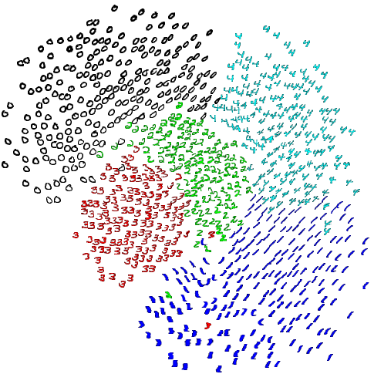
\includegraphics[scale=1.5]{images/image_SNE.png}
% \caption{result of SNE algorithm for UPS dataset}
% \label{fig:label}
% \end{figure}

\section{The Crowding Problem}

As we can observe from the image above, the dimension reduction result is satisfied, which means different kinds of images can be clustered by each category. However, the boundary between each cluster is not clear enough. It would be hard to tell the difference if there is no marks in different color for each group, which is also not convenient for data visualization.\\  

\noindent Part of the reason of this situation is the SNE algorithm pays more attention to the local structure than the global structure. The more important reason could be the difference between the high-dimensional space distance distribution and the low-dimensional space distance distribution. With the increase of the dimensions, the sparseness of high-dimensional spatial data will also increase because the volume increases exponentially.\\

\noindent If there is An $m$-dimensional sphere with radius $r$ centered on data point $x_i$, its space increase with $r^m$. Assuming that the data points are uniformly distributed in the m-dimensional sphere, The distance between other data points and $x_i$ as the dimension increases could be observed as below:

\begin{figure}[ht]

\centering
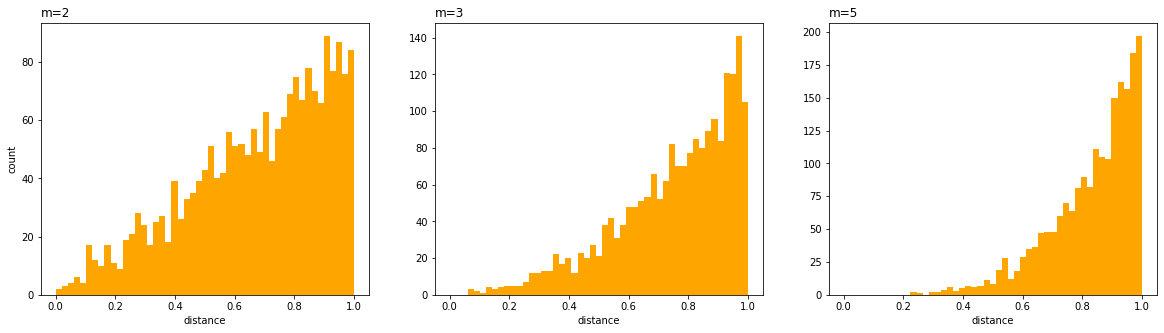
\includegraphics[scale=0.34]{images/image_crowding_problem_1.png}
\caption{distribution of distances between $x_i$ with dimension 2 to 5}
\label{fig:label}
\end{figure}

\begin{figure}[ht]

\centering
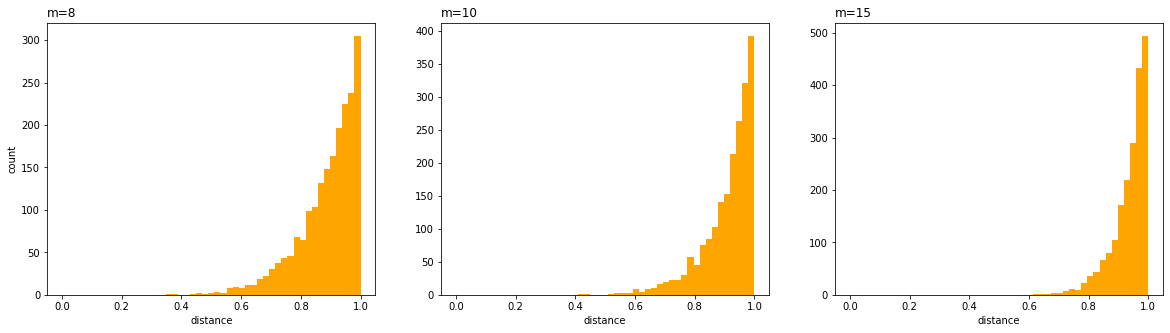
\includegraphics[scale=0.34]{images/image_crowding_problem_2.png}
\caption{distribution of distances between $x_i$ with dimension 8 to 15}
\label{fig:label}
\end{figure}

\noindent It can be observed from the figure that as the dimension increases, most of the data points are clustered near the surface of the sphere, and the distance distribution from the point $x_i$ is extremely uneven. If this distance relationship is directly retained to a low dimension, there will be a crowding problem.

\section{T-SNE}
Draw a random sample with a capacity of $N$ from the normal population. If the mean of the normal population is $μ$, the variance is $\sigma^2$. The mean of the random sample is $\bar{x}$, and the variance is $s^2=  \frac {1}{N−1} \sum ^N_{i=1} (x_i−\bar{x})^2$, and the random variable t can be expressed as:

\begin{equation*}
    {t} =  \frac {\bar{x} - \mu}{s / \sqrt{N}} 
\end{equation*}

\noindent $t$ satisfies the t distribution with n−1 degrees of freedom, written as, $t∼t(n−1)$. t distribution is a typical long-tailed distribution. It is relatively gentle at both ends of the tail, which has obvious advantages when dealing with small samples and abnormal points.\\

\begin{figure}[ht]

\centering
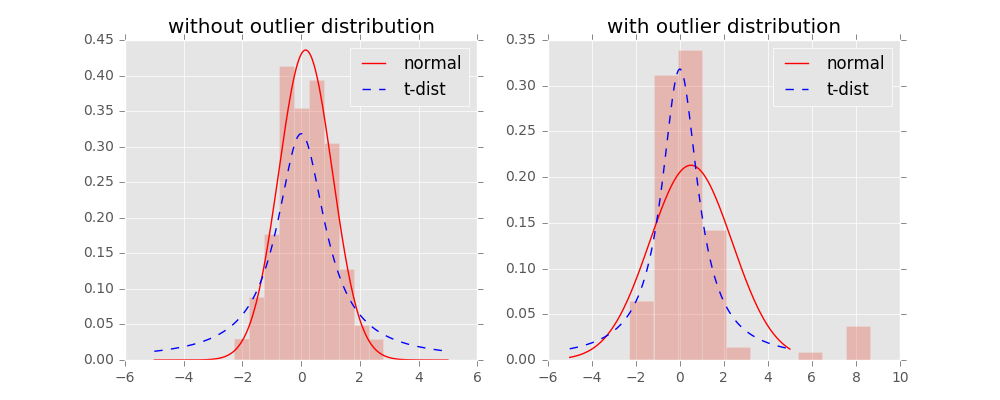
\includegraphics[scale=0.6]{images/image_t-distribution.png}
\caption{normal distribution and t distribution with and with out outliers}
\label{fig:label}
\end{figure}

\noindent From the figure 2.3, it can be easily observed that when there are no outliers, the fitting result of t distribution and Gaussian distribution are basically consistent. In the second picture, there are some abnormal points. Because the tail of the Gaussian distribution is low, it is more sensitive to abnormal points. In order to take care of these abnormal points, the fitting result of the Gaussian distribution deviates from the location of most samples, and the variance is also large. In contrast, the tail of the t distribution is relatively high and it is not sensitive to outliers, that ensure its robustness, so its fitting results are more reasonable, and the overall characteristics of the data are better captured.\\

\noindent With the t distribution now, for points that are close in high-dimensional space, in order to satisfy $p_i_j$=$q_i_j$, the distance in low-dimensional space needs to be slightly smaller; and for points that are far apart in high-dimensional space, in order to satisfy $p_i_j$=$q_i_j$, in low-dimensional space The distance needs to be farther. Then, We redefine the weight function from symmetric SNE: 

\begin{equation*}
    {w_i_j} =  \frac {1}{1+d_i_j^2} 
\end{equation*}

\section{Barnes-Hut t-SNE(BH t-SNE)}

BH t-SNE has some improvements comparing with t-SNE algorithm with the help of tree-based algorithm, including two parts: one is the use of kNN graphs to represent the similarity of points in the high-dimensional space; the other is the optimization of the gradient solution process. The gradient calculation is divided into two parts of gravity and repulsion, and some optimization techniques are also used.

\subsection{kNN graph for the similarity in HD space}

\noindent In t-sne, the overall distance distribution relationship in the high-dimensional space is expressed in the following form:

\begin{equation*}
    {v_{j\mid i}} = \exp {(-\beta_i r^2_{ij})} 
\end{equation*}

\begin{equation*}
    {p_{j\mid i}} = \frac {v_{j\mid i}} {\sum_k^N v_{k\mid i}}
\end{equation*}

\begin{equation*}
    {p_{i j}} = \frac {p_{i\mid j} + p_{j\mid i}} {2N}
\end{equation*}\\

\noindent These three formulas means every data point need to calculate the variance considering all other points. But in fact, the probability $p_i_j$ that two distant points are neighbors to each other is very small and almost negligible. This makes the efficiency of t-SNE is significantly reduced when processing large-scale high-dimensional data.\\

\noindent Therefore, when constructing a distance similarity relationship for a point in a high-dimensional space, it is not necessary to consider every node in the graph, only a number of similar nodes. Here we consider the ⌊3$u$⌋ points closest to the point $x_i$, where $u$ is the perplexity of the conditional probability distribution around the point $x_i$, and only consider the set of these points, which will decrease the amount of calculation. The BH t-SNE algorithm uses a VP tree (vantage-point tree) to construct this kNN graph, and an accurate kNN graph can be obtained within O ($uNlogN$) time complexity.\\

\subsection{Approximation of repulsion in gradient}

When understanding the physical meaning of t-SNE gradient, the gradient can be regarded as the resultant effect of all other points on $y_i$. If $Z$ is set as $Z = \sum_{k \neq l} (1+ \mid y_k−y_l \mid ^2)^{-1}$, then the gradient could be transformed by this feature:

\begin{equation*}
\begin{aligned}
\frac{\partial C_{SSNE}}{\partial y_i} &= {4\sum_j(p_i_j - q_i_j)(y_i - y_j)(1 + \mid y_i - y_j \mid ^ 2) ^{-1}}\\
&= {4\sum_j(p_i_j - q_i_j) (1 + \mid \mid y_i - y_j \mid \mid ^ 2)}
\end{aligned}
\end{equation*}

\begin{equation*}
\begin{aligned}
\frac{\partial C_{SSNE}}{\partial y_i} &= {4(F_{attraction} + F_{repulsion})}\\
&= 4({\sum_{i \neq j}p_i_j q_i_j Z (y_i - y_j)} - {\sum_{i \neq j}q_i_j^2 Z (y_i - y_j)}) 
\end{aligned}
\end{equation*}

\noindent It can be seen that after decomposing the gradient into two parts of attraction and repulsion, the first part is easier to calculate since the $q_i_j Z = 1 + \mid y_i - y_j \mid ^ 2 $ could use the approximation above, which only considers the nearest neighbor nodes, while ignoring distant nodes with time complexity is $O(uN)$. However, there is still a large amount of calculation to calculate repulsion with time complexity $O(N^2)$ because the distribution of $P$ and $Q$ is different, but there are still some optimization techniques to simplify this calculation.\\

\noindent If there are three data points ($y_i,y_j,y_k$) as shown below, their distance relationship can be summarized as $y_i−y_j ≈ y_i−y_k >> y_j−y_k$, the repulsion of $y_j$ and $y_k$ to $y_i$ is approximately equal.

\begin{figure}[ht]

\centering
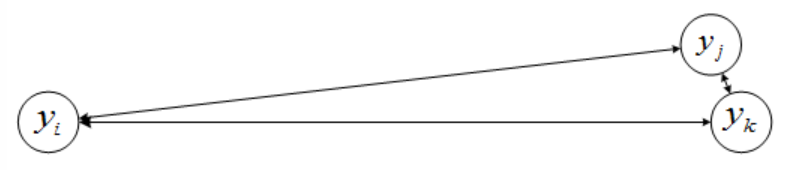
\includegraphics[scale=0.6]{images/image_point_region_1.PNG}
\caption{normal distribution and t distribution with and with out outliers}
\label{fig:label}
\end{figure}

\noindent This situation is very common in low-dimensional space, and even the repulsive force of each point in a certain area can be approximated by the same value. If a point is given arbitrarily, we just need to calculate the repulsion between given point and the centroid of the data points within the certain area, and use the optimization method just now to calculate the total repulsion for them. Of course, not all regions meet this approximate condition. Here, the Barnes-Hut algorithm is used to search and verify the point-region pairs that meet the approximate condition.\\

\subsection{From point-area to area-area}

\noindent In the above approximation, we consider the approximation of the repulsive force between a point and an area. In fact, we can further optimize and consider the approximation of the repulsive force between one area and another area.
\\

\begin{figure}[H]
\centering  %图片全局居中
\subfigure[name1]{
\label{Fig.sub.1}
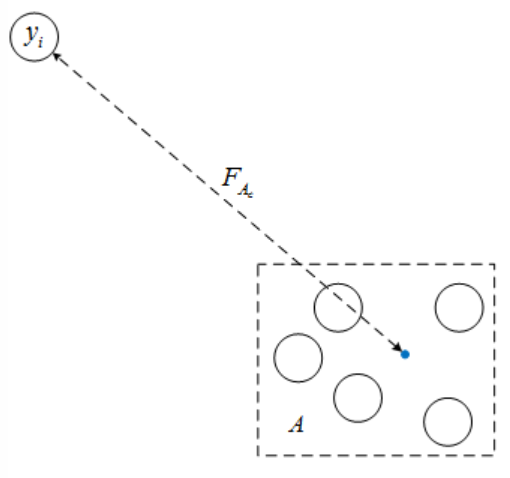
\includegraphics[width=7cm,height=5cm\textwidth]{images/image_point_region_2.PNG}}
\subfigure[name2]{
\label{Fig.sub.2}
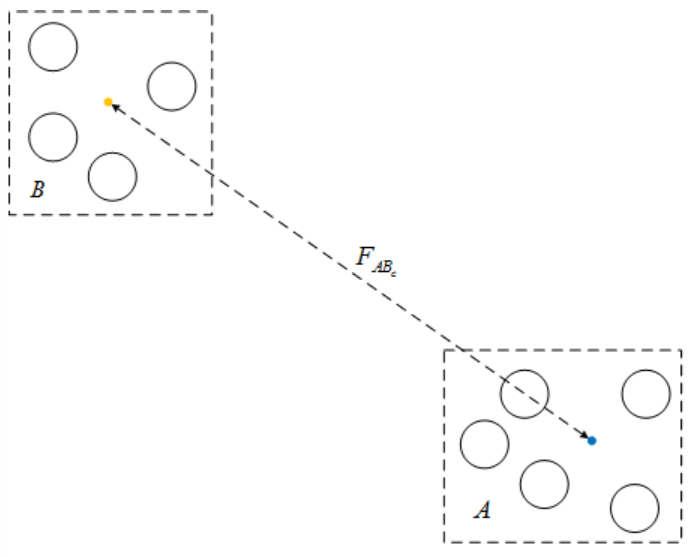
\includegraphics[width=7cm,height=5cm\textwidth]{images/image_region_region_1.PNG}}
\caption{Main name}
\label{Fig.main}
\end{figure}

\noindent Since the result from these two algorithm have similar accuracy and Barnes-Hut T-SNE is much faster than another. This thesis will focus the performance and characteristics of it.

% 再补两个通过bh t-SNE 和 t-SNE 的效果图

\chapter{LargeVis}



\noindent  Although T-SNE works well on small-scale data, there are still some disadvantages of T-SNE:\\

\noindent 1. The efficiency of t-SNE is significantly reduced when processing large-scale high-dimensional data (including BH T-SNE)\\

\noindent 2.The parameters of t-SNE are sensitive to different data sets, which means that even finding out the proper parameters setting for T-SNE in one data set with there is a good visualization effect. However, it cannot be applied to another data set, and it takes a lot of time to find new suitable parameters.\\

\noindent As can be seen from the name, the goal of LargeVis\cite{ref5} is the visualization of large-scale data sets, which takes a different approach comparing with T-SNE: it reuses many of the same definitions as t-SNE but makes sufficiently modified so that stochastic gradient descent can be used. The main improvement is the efficient algorithm for constructing kNN graphs, as well as the low-dimensional space probability calculation formula and objective function.

\section{Efficient kNN graph constructing algorithm}

In the BH t-SNE, for high-dimensional spatial distance similarity, it only consider several neighbor points closest to $x_i$, which is essentially a process of constructing a kNN graph. The VP(vantage-point) tree is used to construct an accurate kNN graph, but the efficiency is still not good, especially for the large-scale dataset. And LargeVis uses a more ingenious way, instead of pursuing a one-step approach, first approximate and then improve accuracy.\\

\subsection{K-D tree and Random Projection Tree}

There are generally three types of common methods for building KNN graph: the first type is the space-partitioning trees algorithm, the second type is the locality sensitive hashing algorithm, and the third type is the neighbor exploring techniques algorithm. Among them, k-d tree and random projection tree belong to the first type of algorithm.\\

\noindent A k-d tree is a data structure that partitions a k-dimensional data space, and is essentially a binary tree. It is mainly used for searching key data in multi-dimensional space, such as range search and nearest neighbor search. The following figure shows the use of k-d trees to search for k nearest neighbors in a two-dimensional space, and then construct a kNN graph. It constructs a kd tree through a recursive process. The root node corresponds to all points in the area. After dividing the space into a left subtree and a right subtree in a certain dimension, the next level of child nodes can be obtained by repeating the splitting process of the root node. Until the number of points corresponding to all leaf nodes in the kd tree is less than a certain threshold.\\

\begin{figure}[ht]

\centering
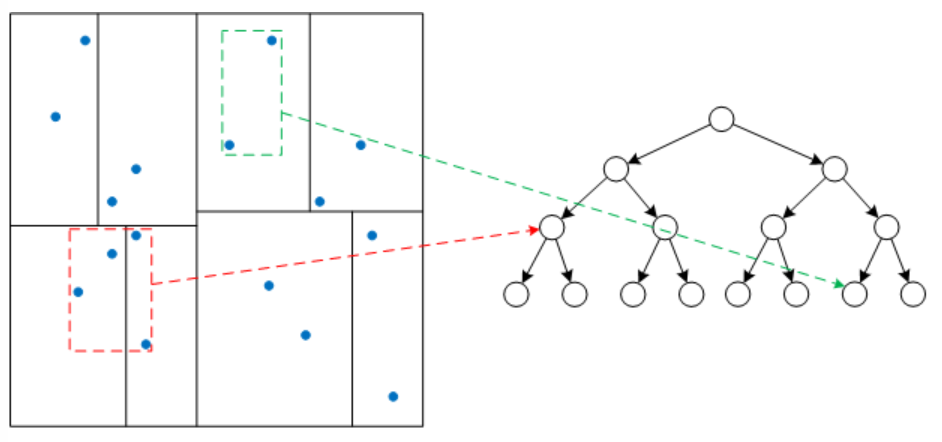
\includegraphics[scale=0.85]{images/image_largevis_k-d_tree_1.PNG}
\caption{k-d tree for dimension 2}
\label{fig:label}
\end{figure}

\noindent With the k-d tree, we don't have to calculate the distance between a certain point and all other points one by one to find k nearest neighbors. For example, to find the k-nearest neighbors of the red dot in the figure below, it only need to search the current subspace, and at the same time, continue to backtrack and search other subspaces of the parent node to find the k-nearest neighbors.\\

\begin{figure}[ht]

\centering
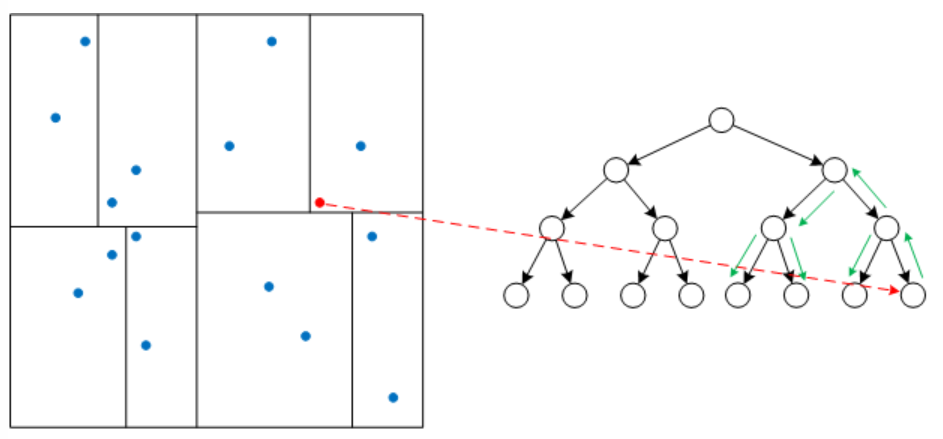
\includegraphics[scale=0.85]{images/image_largevis_k-d_tree_2.PNG}
\caption{finding k-nearest neighbors for k-d tree}
\label{fig:label}
\end{figure}

\noindent However, the biggest problem with the k-d tree is that the way it divides the space is relatively rigid, which is strictly based on the coordinate axis. For high-dimensional data, each dimension of the high-dimensional data is used as a coordinate axis. When the data dimensionality is high, the depth of the k-d tree could be a lot also, which may also lead to the dimensionality disaster problem.\\

\noindent In contrast, the way of dividing the space by random projection trees is more flexible. The basic idea of the random projection tree is similar to the k-d tree, but the way to divide the space is not according to the coordinate axis, but according to the randomly generated unit vector. Because the data in principle is on a manifold, instead of a disorderly manner. Therefore, the depth of the random projection tree is not determined by the dimensionality of the data, but depends on the dimensionality of the manifold where the data is located\cite{ref6}.\\

\begin{figure}[ht]

\centering
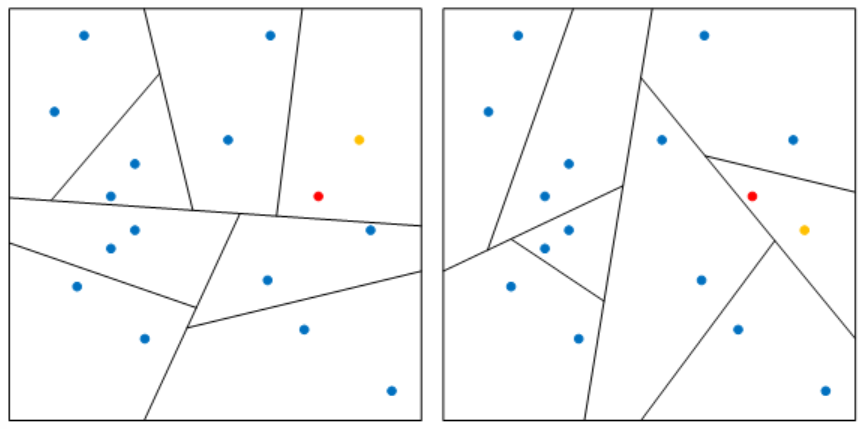
\includegraphics[scale=0.85]{images/image_largevis_random_projection_tree_2.PNG}
\caption{finding k-nearest neighbors for random projection tree}
\label{fig:label}
\end{figure}

\noindent When a random projection tree is used to find k nearest neighbors, the backtracking search method is similar to the k-d tree. If the requirement of the tree's accuracy is not high, the characteristics of the random projection tree can be used to adopt a simpler and time-saving method. That is, we can construct multiple random projection trees in parallel. Since the divided unit vectors are generated randomly, each random projection tree divides the current space differently, as shown in the following figure with two-dimensional space as an example. If the k-nearest neighbors of the red dot need to be fixed, it only need to search the subspace where it is located in different random projection trees, and finally take the union. Although this is time-consuming and space-consuming in the process of constructing a random projection tree, it is very efficient in the search phase.

\subsection{The neighbor’s neighbor may also be my neighbor}

The idea of "neighbors' neighbors may also be my neighbors", starting from an initial nearest-neighbor graph, the algorithm iteratively refines the graph by exploring the neighbors of neighbors defined according to the current graph\cite{ref5}. It use the neighbor search algorithm to find potential neighbors, calculating the distance between the neighbor and the current point, the neighbor's neighbor and the current point, and putting them into a small root pile. Take the k nodes with the smallest distance as k nearest neighbors, and finally get an accurate kNN graph.\\

\section{Low-dimensional space visualization algorithm}

\subsection{Word2vec and Negative sampling}

\noindent After completing the KNN graph algorithm for high dimensional space, we need to project the nodes of the graph into a low-dimensional space. In the process of low-dimensional space visualization, the idea of t-SNE is to ensure that the distance distribution P of the high-dimensional space and the distance distribution Q of the low-dimensional space are as close as possible, and use the KL distance to write the cost function and find the gradient. But the efficiency problem has not been solved well.\\

\noindent In LargeVis algorithm, in order to solve the efficiency problem, a probability model is applied to it to maintain the similarity of vertices in low-dimensional space. That is, the algorithm will bring similar vertices close to each other in a low-dimensional space, and separate different vertices from each other.\\

\subsection{Large-scale Information Network Embedding (LINE) and edge-sampling algorithm}

\chapter{Umap}


testtesttest\\

\chapter{Assessment Algorithm}


testtesttest\\
\part{Comparison} \label{part:Comparison and implementation}

\chapter{comparisons and implementations}

\section{t-SNE}
There are 4 most important parameters for t-SNE, the basic ideas of each parameters are: 

\begin{enumerate}[1)]
\item $perplexity$: number of nearest neighbors for each point
\item $n\_iter$: maximum number of iterations for optimization
\item $early\_exaggeration$: the tightness inside clusters and the distance inbetween
\item $min\_grad\_norm$: the threshold for stopping the optimization 
\end{enumerate}\\

\noindent In order to draw the conclusions in a convincing way, This work examines the three algorithms' quality on several real-world data sets with different level of instances and dimensions, base on the neighborhood-based DR performance criteria discussed above. there are six public databases: Iris, Wine, Breast Cancer Wisconsin Diagnostic (BCW), Optical Recognition of Handwritten Digits test set (Digits), the B. Frey’s images (B.Freys) and Labeled Faces in the Wild face recognition(LFW).\\

\begin{center}
\begin{tabular}{|c|c|c|}% 通过添加 | 来表示是否需要绘制竖线
\hline  % 在表格最上方绘制横线
Datasets & Number of instances & Number of dimensions\\
\hline  %在第一行和第二行之间绘制横线
Iris & 150 & 4\\
\hline  %在第一行和第二行之间绘制横线
Wine & 178 & 13\\
\hline  %在第一行和第二行之间绘制横线
BCW & 569 & 30\\
\hline  %在第一行和第二行之间绘制横线
digit & 1797 & 64\\
\hline  %在第一行和第二行之间绘制横线
B.Freys & 1965 & 560\\
\hline  %在第一行和第二行之间绘制横线
LFW & 13233 & 5749\\
\hline % 在表格最下方绘制横线
\end{tabular}\\
\end{center}
\\

\noindent When we are analyzing the result, we should consider that the high-dimensional sphere was modeled by probability graph, the t-SNE algorithm adapts its "distance" concept to changes in regional density in the data set. As a result, it naturally expands dense clusters and shrinks sparse clusters, making the clusters roughly uniform in size. It also makes it difficult to see the relative size of clusters in the t-SNE graph, and the distance between clusters in low dimensions does not represent the distance between clusters in high dimensions.

\subsection{$perplexity$}

\noindent The first adjustable parameter of t-SNE represent the number of neighbors each point t-SNE considers. It explains how to maintain a balance between the local and global aspects of the data. The perplexity value has a complex effect on the generated pictures, but the performance of SNE is quite reliable for changes in complexity, and the typical value of perplexity is between 5 and 50\cite{ref9}. Also, since the perplexity means the number of the neighbors, it should not be higher than the number of data points.\\

\noindent We can try different potential perplexity values in datasets with different instances. At the same time, since the algorithm using stochastic method, the parameter $random\_state$ is set to 1. This parameter determines the random number generator so that it pass an int mark for reproducible results across multiple function calls. After examining it on the first dataset Iris, we get the figures below:

\begin{figure}[H]
\centering  %图片全局居中
% \subfigure[name1]
{
\label{Fig.sub.1}
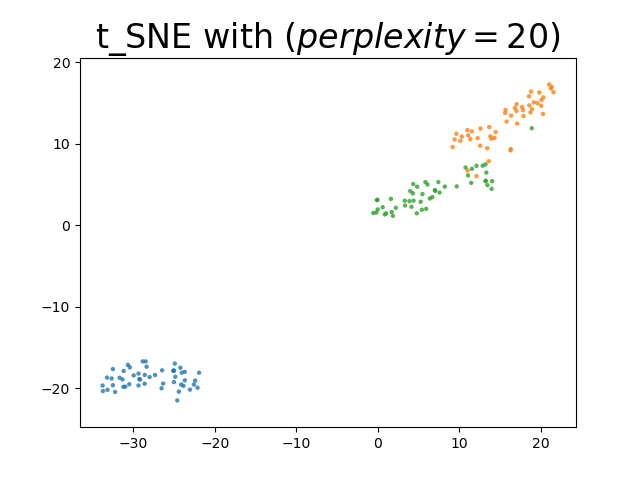
\includegraphics[width=7cm,height=3.5cm\textwidth]{images/image_comparison_tsne_perp20.png}}
% \subfigure[name2]
{
\label{Fig.sub.2}
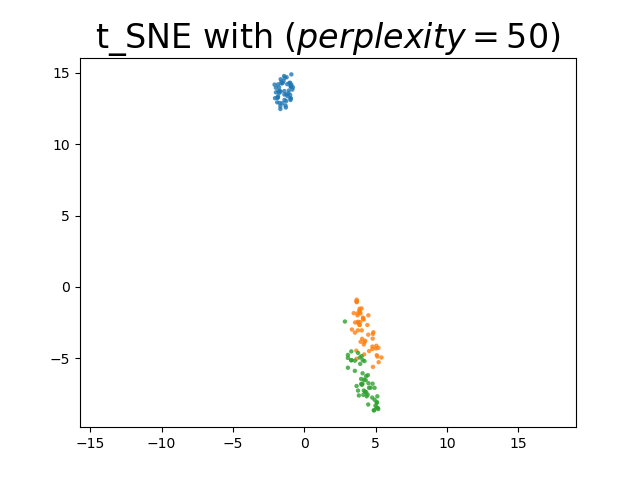
\includegraphics[width=7cm,height=3.5cm\textwidth]{images/image_comparison_tsne_perp50.png}}
% \caption{Main name}
% \label{Fig.main}
\end{figure}

\begin{figure}[H]
\centering  %图片全局居中
% \subfigure[name1]
{
\label{Fig.sub.1}
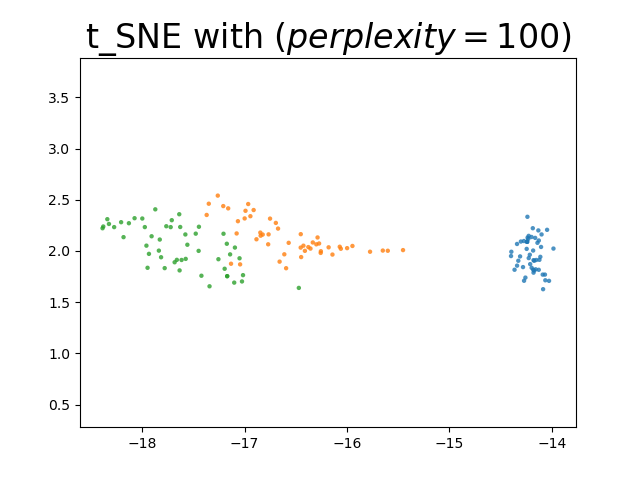
\includegraphics[width=7cm,height=3.5cm\textwidth]{images/image_comparison_tsne_perp100.png}}
% \subfigure[name2]
{
\label{Fig.sub.2}
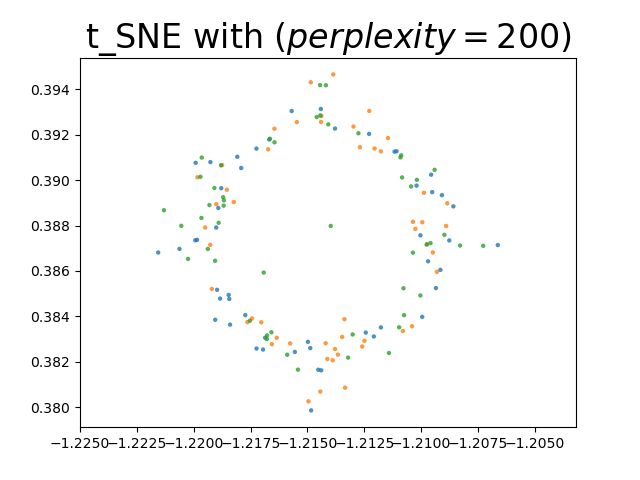
\includegraphics[width=7cm,height=3.5cm\textwidth]{images/image_comparison_tsne_perp200.png}}
\caption{LD result for t-SNE with different perplexity}
% \label{Fig.main}
\end{figure}


\noindent In the figure, we can see that when the value is in the range of 5-50, clusters are well distinguished. Considering that the number of instances of the dataset is only 150, when the value is 100, the clusters begin to merge. When the perplexity = 200, it is difficult to distinguish different clusters. In order for the algorithm to work properly, the perplexity should actually be less than the number of points. Considering the experimental results and the strategy of the search about the optimal number of neighbor from K nearest neighbour algorithm\cite{ref12}, we can simply set perplexity to $n^{0.5}$, where n stand for number of instances. \\

\noindent At the same time, the $AUC$ value for the result with these parameters are 0.731, 0.658, 0.654, -0.004 separately. These $AUC$ values verifies the previous observations. As for the last one, it has a big difference between others and also the only minus result. With the definition of the $R_{NX}$ curve $R_{NX} (K) = ((N − 1)Q_{NX} (K) − K) /(N − 1 − K)$, this is because the K is higher than N in the formula. Numerator is relative small and denominator is a negative number, we then have a minus result.


\subsection{$n\_iter$}

\noindent $n\_iter$ is the maximum number of iterations for the algorithm. The graph observed above are all generated with 1000 iteration which is the default value of $n\_iter$. In principle, the higher $n\_iter$ gives the better result. However, it may be very time consuming when it comes to big dataset. In contrast, if $n\_iter$ is too small, the algorithm does not have enough iteration to generate the convincing clusters in LD. The most important thing is to reach a stable configuration. The figure shows how the result changes with $n\_iter$ grows in the same Iris dataset as above:

\begin{figure}[H]
\centering  %图片全局居中
% \subfigure[name1]
{
\label{Fig.sub.1}
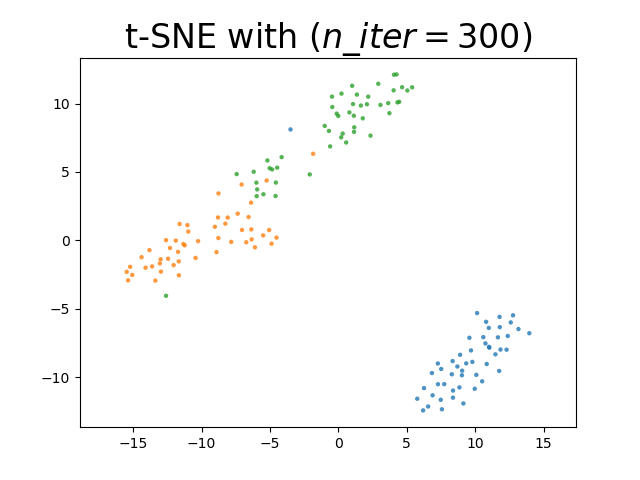
\includegraphics[width=7cm,height=3.5cm\textwidth]{images/t-sne/t-sne_n_iter_300.png}}
% \subfigure[name2]
{
\label{Fig.sub.2}
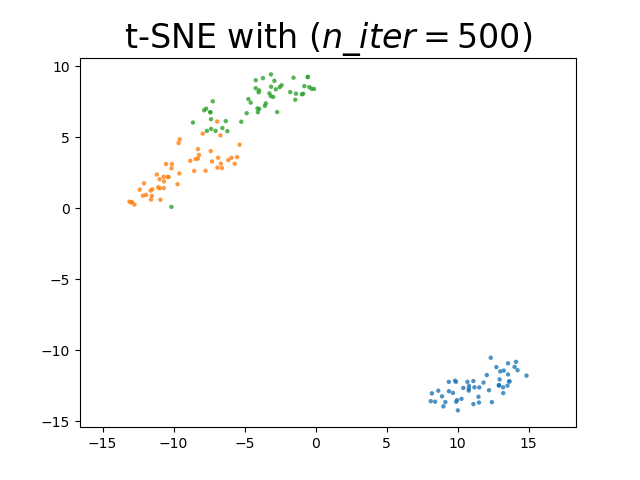
\includegraphics[width=7cm,height=3.5cm\textwidth]{images/t-sne/t-sne_n_iter_500.png}}
\caption{LD result for t-SNE with n\_iter 300 and 500}
% \label{Fig.main}
\end{figure}

\begin{figure}[H]
\centering  %图片全局居中
% \subfigure[name1]
{
\label{Fig.sub.1}
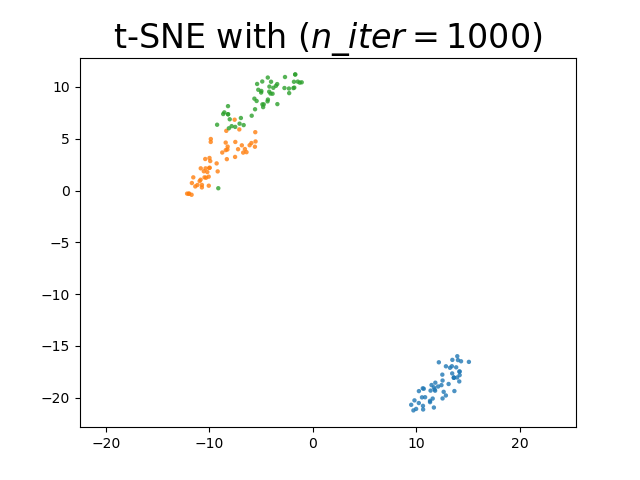
\includegraphics[width=7cm,height=3.5cm\textwidth]{images/t-sne/t-sne_n_iter_1000.png}}
% \subfigure[name2]
{
\label{Fig.sub.2}
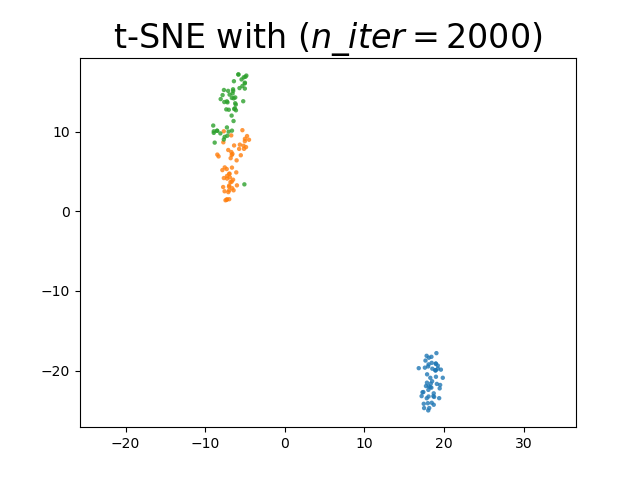
\includegraphics[width=7cm,height=3.5cm\textwidth]{images/t-sne/t-sne_n_iter_2000.png}}
\caption{LD result for t-SNE with n\_iter 1000 and 2000}
% \label{Fig.main}
\end{figure}

\noindent From the figure, we can easily observe that the more iterations, the more well identified for clusters. These four $n\_iter$ generate $AUC$ values for 0.622, 0.654, 0.670, 0.692 separately, which verified the previous conclusion. 

% 上图显示了在困惑度30下的五个不同的运行。前四个在稳定之前已停止。经过10、20、60和120步后,您可以看到带有簇的一维甚至点状图像的布局。如果您看到t-SNE图上有奇怪的“挤压”形状,则该过程可能停止得太早。经过六个不同维度数据集的测试,改参数没有固定的数值可以产生稳定结果。不同的数据集可能需要不同数量的迭代才能收敛。

% 之后还有perp与n_iter之间的heatmap,解释一波

\subsection{$early\_exaggeration$}

$ early\ _exaggeration $ controls the closeness of clusters in high-dimensional space and the distance between them in low-dimensional space. For larger values, the space between natural clusters will be larger in the embedded space. As analyzed before, the distance between the low-dimensional space and the tightness of clustering have limited influence on the result, so this parameter has a small influence on the $AUC$ result. But if the cost function is increased during the initial optimization process, the early exaggeration factor may be too high.

\subsection{$min\_grad\_norm$}

This parameter is the threshold of gradient norm to determine when the optimization will be stopped.

% \bookmarksetup{startatroot}
% \part{Conclusion} \label{part:how is the conclusion}

\chapter{conclusions after comparison}

testtesttest\\

\begin{thebibliography}{99}  
\bibitem{ref1}Nupur Kumari , Siddarth R, Akash Rupela: High-dimensional Data Visualization at Scale, Computer Vision and Pattern Recognition (CVPR), 2012 IEEE Conference on, IEEE, 2012: 2911-2918.  
\bibitem{ref2}Lowe D G. Distinctive image features from scale-invariant keypoints, International journal of computer vision, 2004, 60(2): 91-110.  
\bibitem{ref3}Philbin J, Chum O, Isard M, et al. Lost in quantization: Improving particular object retrieval in large scale image databases, Computer Vision and Pattern Recognition, 2008. CVPR 2008, IEEE Conference on, IEEE, 2008: 1-8.
\bibitem{ref4}J. A. Lee and M. Verleysen. Quality assessment of dimensionality reduction: Rank-based criteria. Neurocomputing, 72(7):1431–1443, 2009.
\bibitem{ref5}Jian Tang, Jingzhou Liu, Ming Zhang, Qiaozhu Mei. Visualizing Large-scale and High-dimensional Data. 2016, the web conference.
\bibitem{ref6}Freund Y, Dasgupta S, Kabra M, et al. Learning the structure of manifolds using random projections[C]. Advances in Neural Information Processing Systems. 2007: 473-480.

\bibitem{ref7}Goldberg Y, Levy O. word2vec explained: Deriving mikolov et al.’s negative-sampling word-embedding method[J]. arXiv preprint arXiv:1402.3722, 2014.

\bibitem{ref8}C de Bodt, D Mulders, M Verleysen, JA Lee Proc. Extensive assessment of Barnes-Hut t-SNE . ESANN, 135-140, 2018.

\bibitem{ref9}L. Van Der Maaten. Accelerating t-SNE using tree-based algorithms. Journal of Machine Learning Research, 15(1):3221–3245, 2014.

\bibitem{ref10}J. A. Lee and M. Verleysen. Nonlinear dimensionality reduction. Springer Science & Business Media, 2007.

\bibitem{ref11}J. A. Lee, E. Renard, G. Bernard, P. Dupont, and M. Verleysen. Type 1 and 2 mixtures of Kullback-Leibler divergences as cost functions in dimensionality reduction based on similarity preservation. Neurocomputing, 112:92–108, 2013.

\bibitem{ref12}Markus Maier, Matthias Hein, Ulrike von Luxburg. Optimal construction of k-nearest-neighbor graphs for identifying noisy clusters.Theor. Comput. Sci, 2009.

\bibitem{ref13}Laurens van der Maaten, Geoffrey Hinton. Visualizing Data using t-SNE. 9(Nov):2579--2605, 2008.

\bibitem{ref14}Rehm F, Klawonn F, Kruse R. MDS polar: a new approach for dimension reduction to visualize high dimensional data[C]//International Symposium on Intelligent Data Analysis. Springer, Berlin, Heidelberg, 2005: 316-327.

\bibitem{ref15}G. Hinton and S. Roweis. Stochastic neighbor embedding. In NIPS, volume 15, pages 833–840, 2002.

\bibitem{ref16}Balasubramanian M, Schwartz E L, Tenenbaum J B, et al. The isomap algorithm and topological stability[J]. Science, 2002, 295(5552): 7-7.

\bibitem{ref17}McInnes L, Healy J, Melville J. Umap: Uniform manifold approximation and projection for dimension reduction[J]. arXiv preprint arXiv:1802.03426, 2018.

\bibitem{ref18}J. A. Lee, E. Renard, G. Bernard, P. Dupont, and M. Verleysen. Type 1 and 2 mixtures of Kullback-Leibler divergences as cost functions in dimensionality reduction based on similarity preservation. Neurocomputing, 112:92–108, 2013.



\end{thebibliography}

  % Back cover page
  \backcoverpage

\end{document}